
\documentclass[12pt,a4paper,landscape]{article}
\usepackage[latin1]{inputenc}
\usepackage{amsmath}
\usepackage{amsfonts}
\usepackage{amssymb}
\usepackage{graphicx}
\usepackage{lscape}
\usepackage{multicol}
\usepackage{setspace}
\usepackage[margin=2.5cm]{geometry}
\newcommand{\est}[2]{\begin{array}[t]{c}
\hspace{-.125in}#1\hspace{-.125in}\vspace{-.13in}\\ 
\hspace{-.125in}#2\hspace{-.125in}
\end{array}}
\linespread{1.6}
\newcommand{\deter}{\ln \mathsf{PE_{t}} =
-     \est{\mathsf{0.077}}{(\mathsf{0.014})}\cos\frac{\pi}{\mathsf{2}}t
+     \est{\mathsf{0.047}}{(\mathsf{0.024})}\sin\frac{\pi}{\mathsf{2}}t
-     \est{\mathsf{0.054}}{(\mathsf{0.007})}(\mathsf{-1})^{t}
+     \mathsf{1.35}    \xi_t
+ \mathsf{N_t}}
\newcommand{\ifmu}{+ \est{\mathsf{0.010}}  {(\mathsf{0.029})}} 
 \newcommand{\nrdiff}{\nabla} 
\newcommand{\ifadf}{ }
\begin{document}
\begin{flushleft}
\thispagestyle{empty}
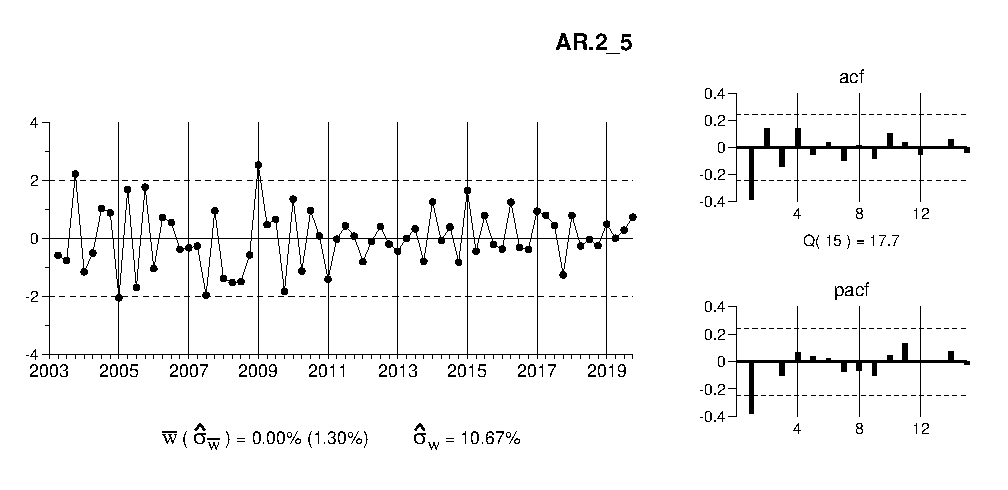
\includegraphics[scale=1]{AR.2_5.eps}
\begin{footnotesize}
$\deter$ \\ 
 $ \left[ 
\nrdiff 
\ifadf \mathsf{N_t} 
\ifmu \right] 
 = \mathsf{AR.2_5_{t}} ; \quad 
\hat{\sigma}_{\mathsf{AR.2_5}}=  \mathsf{ 10.67 } \%  $ 

\bigskip 
\begin{multicols}{2}{ 
\begin{tabular}{ccc}
\hline  Obs.  &  Date &  Std. Val. \\ 
\hline 
 \end{tabular} 
\\ 
 \columnbreak 
 \singlespacing 
 \underline{\textbf{Comments:}} \\ 
 \bigskip       

% \underline{Action:} 
 } 
\end{multicols} 

\end{footnotesize}
\end{flushleft}
\end{document}
